\section*{Introduction}
\label{sec:introduction}

As data becomes cheaper to gather and store, research across a wide range of disciplines has become increasingly reliant on computational workflows involving a familiarity with aspects of statistical modeling, machine learning, scalable computation, and related skills.
At the same time, formal university curricula have been relatively slow to offer courses in these important topics: the slack in this area has often been picked-up by extra-curricular, third-party workshops.
A well-known example is the Software Carpentry and Data Carpentry workshops, whose interdisciplinary workshops in research computing skills have reached more than 16,000 participants since its inception in 1998 \cite{b:wilson-swc-lessons-2016,teal2015data}.
At the same time, there has been a rise in the number of domain-specific courses focusing on statistics and computation within their field.
Examples include the \textit{Summer School in Statistics for Astronomers}\footnote{\url{http://astrostatistics.psu.edu/su16/}}, the Google Earth Engine User Summits\footnote{\url{https://events.withgoogle.com/google-earth-engine-user-summit-2017/}}, and more project-focused than pedagogical meetings, such as the dotAstronomy meetings\footnote{\url{http://dotastronomy.com}}.
Shorter, but similar-spirit meetings have started in conjunction with conferences, such Hack Days at the annual American Astronomical Society meetings, the Brainhack hackathons that take place in conjunction with meetings of the Organization for Human Brain Mapping and the Society for Neuroscience\cite{Cameron_Craddock2016-wc}, and a hackathon associated with the American Geophysical Union meeting\footnote{\url{http://onlinelibrary.wiley.com/doi/10.1002/2014EO480004/pdf}}.
In broad-brush, pedagogically-focused workshops and summer schools tend to follow a classic academic model where novices learn a skillset from experts, while project-focused workshops focus on people collaboratively exercising the skillset they already have.
A disadvantage of the summer school model is that it can tends to focus on a one-way flow of information from instructor to student, and can discount the potential contributions by students.
A disadvantage of the hackathon model is the common perception (whether accurate or not) that the week is designed for experts in technical tools, which may discourage others from attending.
In 2014, we started Astro Hack Week to try to fill the gaps between these models.
The hack week model combines pedagogy (often focused on statistical and computational techniques) with room for collaborative hacks or creative projects, with the goal of encouraging collaboration and learning among people at various stages of their career.

\begin{figure}
\begin{center}
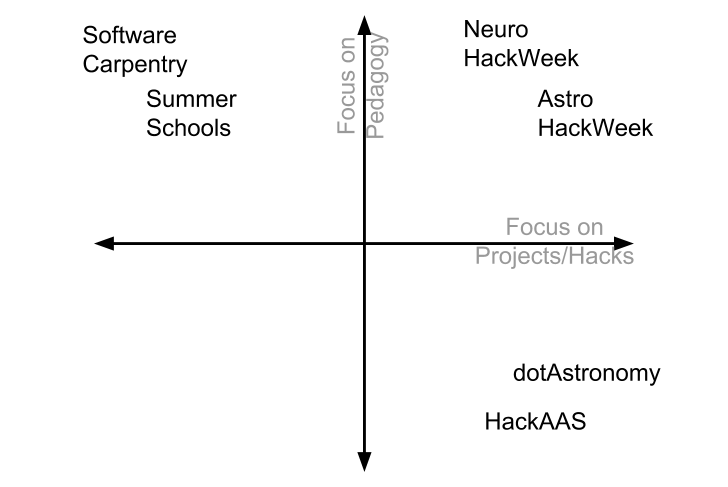
\includegraphics[width=9cm]{fig/HackSpectrum}
\caption{Comparison of Extracurricular Workshop Models}
\label{fig:hackspectrum}
\end{center}
\end{figure}

As of the publication of this paper, we have run eight such hack week events: four focused on Astronomy, two focused on Neuroscience, and two focused on Geoscience.
Below we will share some of the philosophy behind the hack week model, practical lessons we have learned in organizing these events, and recommendations for future hack weeks in other disciplines.
